\chapter{Introduction}
\section{Notation}

\section{Block ciphers}

Securing communication channels between different parties has been a long-term
subject of study for cryptographers and engineers which is essential to our
modern world to cope with ever-increasing amounts of devices producing and
sharing data. The main way to facilitate high-throughput, confidential
communications nowadays is through the use of symmetric cryptography in which
two parties share a common secret, called a key, which allows them to encrypt,
share and subsequently decrypt messages to achieve confidentiality against
third parties. Ciphers can be divided into two categories; block ciphers, which
always encrypt fixed-sized messages called blocks, and stream ciphers, which
continuously provide encryption for an arbitrarily long, constant stream of
data.

A block cipher can be defined as a bijection between the input block (the
message) and the output block (the ciphertext). For any block cipher with block
size $n$, we denote the key-dependent encryption and decryption functions as
$E_K,D_K:\F{n}\rightarrow \F{n}$. The simplest way to
characterize this bijection is through a lookup table which yields the highest
possible performance as each block can be encrypted by one simple lookup
depending on the key and the message. This is not practical though due to most
ciphers working with block and key sizes $n,|K|\geq 64$. For a block cipher
with $n=64,|K|=128$, a space of $2^{64}2^{128}64=2^{198}$ is necessary.
Considering modern consumer hard disks being able to store data in the order of
$2^{40}$, it is easy to see that a lookup table is wholly impractical. We
therefore describe block ciphers algorithmically which opens up possibilities
for different tradeoffs and security concerns.


\subsection{GIFT}

\texttt{GIFT}\cite{gift:2017}, first presented in the \textit{CHES 2017}
cryptographic hardware and embedded systems conference, is a lightweight block
cipher based on a previous design called \texttt{PRESENT}, developed in 2007. Its
goal is to offer maximum security while being extremely light on resources.
Modern battery-powered devices like RFID tags or low-latency operations like
on-the-fly disc encryption present strong hardware and power constraints. GIFT
aims to be a simple, low-energy cipher suited for these kinds of applications.

\texttt{GIFT} comes in two variants; \verb|GIFT-64| working with 64-bit blocks
and GIFT-128 working with 128-bit blocks. In both cases, the key is 128
bits long. The design is a very simple, round-based substitution-permutation
network (SPN). One round consists in a sequential application of the confusion
layer by means of 4-bit S-boxes and subsequent diffusion through bit
permutation. After the bit permutation, a round key is added to the cipher
state and the single round is complete. GIFT-64 uses 28 rounds while
GIFT-128 uses 40 rounds.

\begin{figure}[h!]
    \centering
    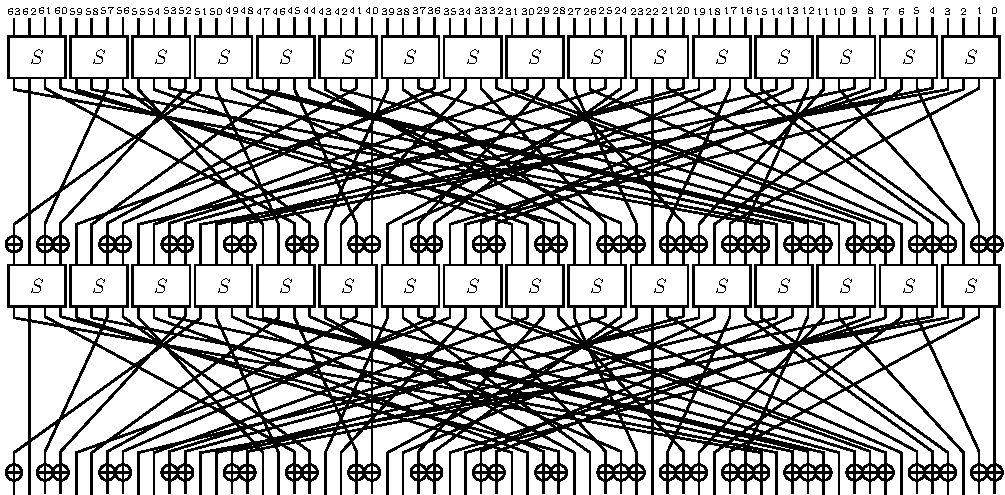
\includegraphics[width=\textwidth]{Figures/GIFT-64.pdf}
    \caption{Two rounds of GIFT-64}
\end{figure}

\subsubsection{Substitution layer}

The input of \texttt{GIFT} is split into 4-bit nibbles which are then fed into
16 S-boxes for GIFT-64 and 32 S-boxes for GIFT-128. The S-box
$S:\F{4}\rightarrow \F{4}$ is defined as follows:

\[
    \begin{array}{l|cccccccccccccccc}
        x & 0 & 1 & 2 & 3 & 4 & 5 & 6 & 7 & 8 & 9 & a & b & c & d & e & f \\
        \hline
        S(x) & 1 & a & 4 & c & 6 & f & 3 & 9 & 2 & d & b & 7 & 5 & 0 & 8 & e
    \end{array}
\]

\subsubsection{Permutation layer}

The permutation $P$ works on individual bits and maps bit $b_i$ to $b_{P(i)}$.
The different permutations for GIFT-64 and GIFT-128 can be expressed by:

\begin{align*}
    P_{64}(i)&=4\left\lfloor\frac{i}{16}\right\rfloor+16\left(\left(3\left\lfloor\frac{i\bmod 16}{4}\right\rfloor+(i\bmod 4)\right)\bmod 4\right)+(i\bmod 4) \\
    P_{128}(i)&=4\left\lfloor\frac{i}{16}\right\rfloor+32\left(\left(3\left\lfloor\frac{i\bmod 16}{4}\right\rfloor+(i\bmod 4)\right)\bmod 4\right)+(i\bmod 4) \\
\end{align*}

\subsubsection{Round key addition}

The last step of each round consists in XORing a round key $R_{i}$ to the cipher
state. The new cipher state $x_{i+1}$ after each full round is therefore given
by

\[
    x_{i+1}=P(S(x_i))\oplus R_i
\]

\subsubsection{Round key extraction and key schedule}

Round key extraction differs for GIFT-64 and GIFT-128. Let
$K_{(128)}=k_7||k_6||\dots||k_0$ denote the 128-bit key state.

\paragraph{GIFT-64}. We extract two words $U_{(16)}||V_{(16)}=k_1||k_0$ from the key
state. These are then added to round key $R_{(64)}$: $R_{4i+1}\leftarrow
U_i,R_{4i}\leftarrow V_i$.

\paragraph{GIFT-128}. We extract two words
$U_{(32)}||V_{(32)}=k_5||k_4||k_1||k_0$ from the key state. These are then
added to round key $R_{(128)}$: $R_{4i+2}\leftarrow U_i,R_{4i+1}\leftarrow
V_i$.

In both cases, we additionally XOR a round constant $C_{(6)}$ to bit positions
$n-1,23,19,15,11,7,3$. The round constants are generated using a 6-bit affine
linear-feedback shift register and have the following values:\\

\begin{tabular}{r|l}
    \textbf{Rounds} & \textbf{Constants} \\
    \hline
    \textbf{1 - 16} &  \small\texttt{01,03,07,0F,1F,3E,3D,3B,37,2F,1E,3C,39,33,27,0E} \\
    \textbf{17 - 32} & \small\texttt{1D,3A,35,2B,16,2C,18,30,21,02,05,0B,17,2E,1C,38} \\
    \textbf{33 - 48} & \small\texttt{31,23,06,0D,1B,36,2D,1A,34,29,12,24,08,11,22,04}
\end{tabular}\\

The key state is then updated by individually rotating $k_1$ and $k_0$ and
rotating the new state $32$ bits to the right:

\[
    k_7||k_6||\dots||k_1||k_0\leftarrow k_1\ggg 2||k_0\ggg 12||k_7||k_6||\dots||k_3||k_2
\]

\subsection{Camellia}

Camellia\cite{camellia:2001} is a block cipher jointly developed by NTT and
Mitsubishi Electric Corporation and first published in 2001. Following AES
specifications, it is able to encrypt 128-bit blocks using either 128-, 196- or
256-bit keys and claims to possess similar performance and security levels as
the AES finalists.

\subsubsection{Encryption}

The encryption process has an 18-round Feistel structure for 128-bit keys and a
24-round Feistel structure for 192/256-bit key and employs key whitening to
increase security. First, subkeys $kw_{t(64)}(t=0,1,2,3)$,
$k_{u(64)}(u=0,1,\dots,(17|23)$ and $kl_{v(64)}(v=0,1,2,3)$ are generated from
the master key. Then, pre-whitening keys are applied to the plaintext
$m_{(128)}=L_{(64)}||R_{(64)}$:

\[
    (L||R)\leftarrow (L||R)\oplus (kw_0||kw_1)
\]

The next steps differ for 128-bit and 192/256-bit keys in the number of rounds:

\begin{table}[h!]
    \centering
    \caption{Camellia encryption}
    \begin{tabular}{lll}
        \toprule
        Round $r$ & 128-bit keys & 192/256-bit keys \\
        \midrule
        0-4 & $(L||R)\leftarrow FE(L,R,k_r)$ & $(L||R)\leftarrow FE(L,R,k_r)$ \\
        \midrule
        5 & {$\!\begin{aligned}&(L||R)\leftarrow FE(L,R)\\&(L||R)\leftarrow FLL(L,R,kl_0,kl_1)\end{aligned}$} & {$\!\begin{aligned}&(L||R)\leftarrow FE(L,R)\\&(L||R)\leftarrow FLL(L,R,kl_0,kl_1)\end{aligned}$} \\
        \midrule
        6-10 & $(L||R)\leftarrow FE(L,R,k_r)$ & $(L||R)\leftarrow FE(L,R,k_r)$ \\
        \midrule
        11 & {$\!\begin{aligned}&(L||R)\leftarrow FE(L,R)\\&(L||R)\leftarrow FLL(L,R,kl_2,kl_3)\end{aligned}$} & {$\!\begin{aligned}&(L||R)\leftarrow FE(L,R)\\&(L||R)\leftarrow FLL(L,R,kl_2,kl_3)\end{aligned}$} \\
        \midrule
        12-16 & $(L||R)\leftarrow FE(L,R,k_r)$ & $(L||R)\leftarrow FE(L,R,k_r)$ \\
        \midrule
        17 & & {$\!\begin{aligned}&(L||R)\leftarrow FE(L,R)\\&(L||R)\leftarrow FLL(L,R,kl_4,kl_5)\end{aligned}$} \\
        \midrule
        18-23 & & $(L||R)\leftarrow FE(L,R,k_r)$ \\
        \bottomrule
    \end{tabular}
\end{table}

Finally, $R$ and $L$ are concatenated and XORed with the post-whitening keys to
obtain the cipher text $c_{(128)}$:

\[
    c=(R||L)\oplus (kw_2)||kw_3)
\]

\subsubsection{Key schedule}

The master key $K$ is split into two parts $K=K_{L(128)}||K_{R(128)}$ with
$K_R=0$ for 128-bit keys. Then, two variables $K_{A(128)},K_{B(128)}$ are
generated by repeated application of the round function with key constants
$\Sigma_i,i=(0,1,\dots,5)$:

\begin{align*}
    K_A&\leftarrow K_L\oplus K_R \\
    K_A&\leftarrow FE(FE(K_A, \Sigma_0\mathrm{0xa09e667f3bcc908b}), \Sigma_1\mathrm{0xb67ae8584caa73b2}) \\
    K_A&\leftarrow K_A\oplus K_L \\
    K_A&\leftarrow FE(FE(K_A, \Sigma_2\mathrm{0xc6ef372fe94f82be}), \Sigma_3\mathrm{0x54ff53a5f1d36f1c}) \\
    K_B&\leftarrow FE(FE(K_A, \Sigma_4\mathrm{0x10e527fade682d1d}), \Sigma_5\mathrm{0xb05688c2b3e6c1fd})
\end{align*}

Subkeys are then created by rotating $K_L,K_R,K_A,K_B$:

\begin{table}[h!]
    \centering
    \scriptsize
    \caption{Subkey creation for 128-bit keys}
    \begin{tabular}{lll|lll}
        \toprule
        Usage & Subkey & Value & Usage & Subkey & Value \\
        \midrule
        \multirow{2}{*}{Prewhitening} & $kw_{0(64)}$ & $(K_L{\lll_0})_{L(64)}$ & $F(\text{Round 9})$ & $k_{9(64)}$ & $(K_L{\lll_{60}})_{R(64)}$ \\
                                      & $kw_{1(64)}$ & $(K_L{\lll_0})_{R(64)}$ & $F(\text{Round 10})$ & $k_{10(64)}$ & $(K_A{\lll_{60}})_{L(64)}$ \\
        $F(\text{Round 0})$ & $k_{0(64)}$ & $(K_A{\lll_0})_{L(64)}$            & $F(\text{Round 11})$ & $k_{11(64)}$ & $(K_A{\lll_{60}})_{R(64)}$ \\
        $F(\text{Round 1})$ & $k_{1(64)}$ & $(K_A{\lll_0})_{R(64)}$            & $FL$        & $kl_{2(64)}$ & $(K_L{\lll_{77}})_{L(64)}$ \\
        $F(\text{Round 2})$ & $k_{2(64)}$ & $(K_L{\lll_{15}})_{L(64)}$         & $FL^{-1}$   & $kl_{3(64)}$ & $(K_L{\lll_{77}})_{R(64)}$ \\
        $F(\text{Round 3})$ & $k_{3(64)}$ & $(K_L{\lll_{15}})_{R(64)}$         & $F(\text{Round 12})$ & $k_{12(64)}$ & $(K_L{\lll_{94}})_{L(64)}$ \\
        $F(\text{Round 4})$ & $k_{4(64)}$ & $(K_A{\lll_{15}})_{L(64)}$         & $F(\text{Round 13})$ & $k_{13(64)}$ & $(K_L{\lll_{94}})_{R(64)}$ \\
        $F(\text{Round 5})$ & $k_{5(64)}$ & $(K_A{\lll_{15}})_{R(64)}$         & $F(\text{Round 14})$ & $k_{14(64)}$ & $(K_A{\lll_{94}})_{L(64)}$ \\
        $FL$        & $kl_{0(64)}$ & $(K_A{\lll_{30}})_{L(64)}$                & $F(\text{Round 15})$ & $k_{15(64)}$ & $(K_L{\lll_{94}})_{R(64)}$ \\
        $FL^{-1}$   & $kl_{1(64)}$ & $(K_A{\lll_{30}})_{R(64)}$                & $F(\text{Round 16})$ & $k_{16(64)}$ & $(K_A{\lll_{111}})_{L(64)}$ \\
        $F(\text{Round 6})$ & $k_{6(64)}$ & $(K_L{\lll_{45}})_{L(64)}$         & $F(\text{Round 17})$ & $k_{17(64)}$ & $(K_A{\lll_{111}})_{R(64)}$ \\
        $F(\text{Round 7})$ & $k_{7(64)}$ & $(K_L{\lll_{45}})_{R(64)}$         & \multirow{2}{*}{Postwhitening} & $kw_{2(64)}$ & $(K_A{\lll_{111}})_{L(64)}$ \\
        $F(\text{Round 8})$ & $k_{8(64)}$ & $(K_A{\lll_{45}})_{L(64)}$         &                                & $kw_{3(64)}$ & $(K_A{\lll_{111}})_{R(64)}$ \\
        \bottomrule
    \end{tabular}
\end{table}

Subkeys for 192/256-bit keys are generated in a similar way.

\subsubsection{Components}

We will give an overview of the main functional components of Camellia.

\begin{description}
\item[Feistel round function $FE$:]

\begin{align*}
    FE:(\F{64})^3 &\rightarrow (\F{64})^2 \\
    (L_{(64)},R_{(64)},k_{(64)})&\mapsto (R\oplus F(L,k), L)
\end{align*}

\item[SP-function $F$:]

\begin{align*}
    F:(\F{64})^2 &\rightarrow \F{64} \\
    (X_{(64)},k_{(64)})&\mapsto P(S(X\oplus k))
\end{align*}

\item[Substitution function $S$:]

\begin{align*}
    S:\F{64} &\rightarrow \F{64} \\
    \begin{aligned}
        l_{0(8)}||l_{1(8)}||l_{2(8)}||l_{3(8)}&||\\
        l_{4(8)}||l_{5(8)}||l_{6(8)}||l_{7(8)}&
    \end{aligned}&\mapsto
    \begin{aligned}
        s_0(l_0)||s_1(l_1)||s_2(l_2)||s_3(l_3)&||\\
        s_1(l_4)||s_2(l_5)||s_3(l_6)||s_0(l_7)&
    \end{aligned},
\end{align*}

with 8-bit S-boxes $s_0,s_1,s_2,s_3:\F{8}\rightarrow \F{8}$.

\item[Permutation function $P$:]

\begin{align*}
    P:\F{64} &\rightarrow \F{64} \\
    \begin{pmatrix}z_7\\z_6\\z_5\\z_4\\z_3\\z_2\\z_1\\z_0\end{pmatrix}&\mapsto
    \begin{pmatrix}
        0 & 1 & 1 & 1 & 1 & 0 & 0 & 1 \\
        1 & 0 & 1 & 1 & 1 & 1 & 0 & 0 \\
        1 & 1 & 0 & 1 & 0 & 1 & 1 & 0 \\
        1 & 1 & 1 & 0 & 0 & 0 & 1 & 1 \\
        0 & 1 & 1 & 1 & 1 & 1 & 1 & 0 \\
        1 & 0 & 1 & 1 & 0 & 1 & 1 & 1 \\
        1 & 1 & 0 & 1 & 1 & 0 & 1 & 1 \\
        1 & 1 & 1 & 0 & 1 & 1 & 0 & 1
    \end{pmatrix}\begin{pmatrix}z_7\\z_6\\z_5\\z_4\\z_3\\z_2\\z_1\\z_0\end{pmatrix}
\end{align*}

\item[$FL$ layer function $FLL$:]

\begin{align*}
    FLL:(\F{64})^4 &\rightarrow (\F{64})^2 \\
    (X_{L(64)},X_{R(64)},k_{0(64)},k_{1(64)})&\mapsto (FL(X_L,k_0),FL^{-1}(X_R,k_1))
\end{align*}

\item[$FL$:]

\begin{align*}
    FL:(\F{64})^2 &\rightarrow \F{64} \\
    (X_{L(32)}||X_{R(32)},k_{L(32)}||k_{R(32)})&\mapsto (Y_{L(32)}||Y_{R(32)}),
\end{align*}

where

\begin{align*}
    Y_{R(32)}&=((X_L\cap k_{L})\lll_1)\oplus X_{R} \\
    Y_{L(32)}&=(Y_R\cup k_{R})\oplus X_{L}
\end{align*}

\item[$FL^{-1}$:]

\begin{align*}
    FL^{-1}:(\F{64})^2 &\rightarrow \F{64} \\
    (Y_{L(32)}||Y_{R(32)},k_{L(32)}||k_{R(32)})&\mapsto (X_{L(32)}||X_{R(32)}),
\end{align*}

where

\begin{align*}
    X_{L(32)}&=(Y_R\cup k_{R})\oplus Y_{L} \\
    X_{R(32)}&=((X_L\cap k_{L})\lll_1)\oplus Y_{R}
\end{align*}
\end{description}

\section{The ARMv8 platform}

With small devices and embedded processors becoming ever more ubiquitous and
essential in areas like consumer electronics or industrial and IoT
applications, the need for low-power, high-performance microprocessors has
increased steadily. With more than 250 billion chips shipped, semiconductors
designed by ARM power 95\% of mobile devices and have found a great many
applications due to their high performance and low power
consumption\cite{armcompany}. The ODROID-N2+\cite{odroidn2} development board
we are using is based on the big.LITTLE architecture and is powered by a
quad-core ARM Cortex-A73 processor and a weaker dual-core ARM Cortex-A53 for
power efficiency. Both these processors are part of the eight generation of ARM
designs known as ARMv8\cite{armv8:2013}.

ARMv8 defines three architecture profiles for different use cases as well as
dynamic execution states with corresponding instruction sets. This work will
focus on the A profile running in the AArch64 state utilizing the A64
instruction set with NEON and crypto extensions.

\begin{table}[h!]
    \centering
    \caption{ARMv8 profiles}
    \begin{tabularx}{\textwidth}{lX}
        \toprule
        Profile & Description \\
        \midrule
        Application (A) & Traditional use with virtual memory and privilege level support \\
        Real-time (R) & Real-time, low-latency, deterministic embedded systems \\
        Microcontroller (M) & Very low-power, fast-interrupt embedded systems \\
        \bottomrule
    \end{tabularx}
\end{table}

\begin{table}[h!]
    \centering
    \caption{ARMv8 execution states}
    \begin{tabularx}{\textwidth}{llX}
        \toprule
        Execution state & Usage & Instruction sets \\
        \midrule
        AArch32 & 32-bit compatibility & A32/T32 \\
        AArch64 & 64-bit & A64 \\
        \bottomrule
    \end{tabularx}
\end{table}

\subsection{General architecture}

ARMv8 is a RISC architecture employing simple data processing instructions
operating only on registers as well as dedicated load/store instructions to
transfer data from register to memory and back. This enables faster execution
of individual instructions, a simplier pipeline design, predictable instruction
timings and fewer addressing modes.

The A64 instruction set defines 31 64-bit general-purpose registers
\texttt{X0-X30} which can also be accessed as 32-bit registers \texttt{W0-W30}.
Values are loaded from and stored to memory using \texttt{LDR}/\texttt{STR}.
Data processing instructions generally use explicit output registers instead of
overwriting the first input register.

\begin{table}[h!]
    \centering
    \small
    \caption{A64 addressing modes}
    \begin{tabularx}{\textwidth}{llX}
        \toprule
        Addressing mode & Example & Description \\
        \midrule
        Base register & \texttt{LDR W0, [X1]} & \texttt{W0 = *(X1);} \\
        Offset & \texttt{LDR W0, [X1, \#12]} & \texttt{W0 = *(X1 + 12);} \\
        Pre-indexing & \texttt{LDR W0, [X1, \#12]!} & \texttt{X1 += 12; W0 = *(X1);} \\
        Post-indexing & \texttt{LDR W0, [X1], \#12} & \texttt{W0 = *(X1); X1 += 12;} \\
        \bottomrule
    \end{tabularx}
\end{table}

\subsection{NEON}
\label{ss:neon}

ARMv8 supports single-instruction, multiple-data (SIMD) processing. These systems
allow the programmer to store multiple pieces of data in a vector and work on
them in parallel to speed up calculations. The A64 instruction set defines two
possible SIMD implementations:

\begin{enumerate}
    \item Advanced SIMD, known as NEON
    \item Scalable Vector Extension (SVE)
\end{enumerate}

We will take a look at NEON as this is the type of vector processing supported
by the Cortex-A73 processor.

The register file of the NEON unit is made up of 32 quad-word (128-bit)
registers \texttt{V0-V31}, each extending the standard 64-bit floating-point
registers \mbox{\texttt{D0-31}}. These registers are divided into equally sized
lanes on which vector instructions operate. Figure \ref{fig:regdivs} shows
valid ways to interpret the register \texttt{V0}.

\begin{figure}[h!]
    \centering
    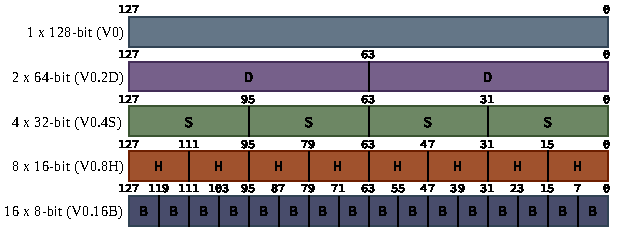
\includegraphics[width=\textwidth]{Figures/V_register.pdf}
    \caption{Divisions of the V0 register}
    \label{fig:regdivs}
\end{figure}

NEON instructions interpret their operands' layouts (i.e. lane count and width)
through the use of suffixes such as \texttt{.4S} or \texttt{.8H}. Adding eight
16-bit halfwords stored in \texttt{V1} and \texttt{V2} can be done as follows:

\begin{center}
    \texttt{ADD V0.8H, V1.8H, V2.8H}
\end{center}

\begin{figure}[h!]
    \centering
    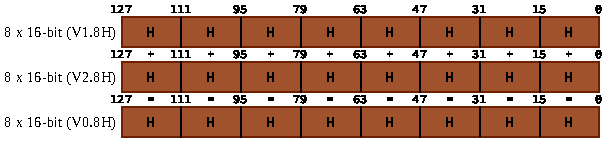
\includegraphics[width=\textwidth]{Figures/vector_add.pdf}
    \caption{Addition of two vector registers}
\end{figure}

\subsection{NEON Intrinsics}

The header file \texttt{<arm\_neon.h>} provides ARM-specific data and function
definitions including vector data types and C functions for working with these
vectors. These functions are known as NEON intrinsics \cite{neonintr:2022} and
give the programmer a high-level interface to most NEON instructions. Major
advantages of this approach include the ease of development as the compiler
takes over register allocation and load/store operations as well as performance
benefits through compiler optimizations.

Standard vector data types have the format \texttt{uintnxm\_t} with lane width
$n$ in bits and and lane count $m$. Array types of the format
\texttt{uintnxmxc\_t}, $c\in\{2,3,4\}$ are also defined which are used in
operations requiring multiple parameters like \texttt{TBL} or pairwise
load/stores. Intrinsics include the operation name and lane data format as well
as an optional \texttt{q} suffix to indicate operation on a 128-bit register.
Multiplying eight pairs of 16-bit numbers \texttt{a,b} for example can be done
via the following:

\begin{center}
    \texttt{uint16x8\_t result = vmulq\_u16(a, b);}
\end{center}

In this case, the compiler allocates vector registers for \texttt{a},
\texttt{b} and \texttt{result} and assembles the intrinsic to \texttt{MUL
Vr.8H, Va.8H, Vb.8H}. Necessary loads and stores for the result and parameters
are also handled automatically. Of special interest to us are the following
intrinsics, each existing in different variants with different lane widths and
also array types: \\

\begin{table}[h!]
    \centering
    \footnotesize
    \caption{Common NEON intrinsics}
    \begin{tabularx}{\textwidth}{llX}
        \toprule
        Intrinsic && Summary \\
        \midrule
        \texttt{uint64\_t} & \texttt{vgetq\_lane\_u64(void)} & Extract a single lane \\
        \midrule
        \texttt{void} & \texttt{vsetq\_lane\_u64(uint64\_t)} & Insert a single lane \\
        \midrule
        \texttt{uint64x2\_t} & \texttt{vdupq\_n\_u64(uint64\_t)} & Initialize all lanes to same value \\
        \midrule
        \texttt{void} & \texttt{vst1q\_u64(uint64\_t*, uint64x2\_t)} & Store from register to memory \\
        \midrule
        \texttt{uint64x2\_t} & \texttt{vld1q\_u64(uint64\_t*, uint64x2\_t)} & Load from memory to register \\
        \midrule
        \texttt{uint8x16\_t} & \texttt{veorq\_u8(uint8x16\_t, uint8x16\_t)} & bitwise XOR \\
        \midrule
        \texttt{uint8x16\_t} & \texttt{vandq\_u8(uint8x16\_t, uint8x16\_t)} & bitwise AND \\
        \midrule
        \texttt{uint8x16\_t} & \texttt{vorrq\_u8(uint8x16\_t, uint8x16\_t)} & bitwise OR \\
        \midrule
        \texttt{uint8x16\_t} & \texttt{vmvnq\_u8(uint8x16\_t)} & bitwise NOT \\
        \midrule
        \texttt{uint8x16\_t} & \texttt{vqtbl2q\_u8(uint8x16\_t, uint8x16\_t)} & permutation (\texttt{TBL}) \\
        \midrule
        \texttt{uint64x2\_t} & \texttt{vextq\_u64(uint64x2\_t, uint64x2\_t, int)} & extract from pair of vectors \\
        \bottomrule
    \end{tabularx}
\end{table}
